\section{نظریه اطلاعات}
 در سال ۱۹۴۸ شنون\LTRfootnote{Claude Shannon} در مقاله‌ای با عنوان 
\href{https://web.archive.org/web/19980715013250/http://cm.bell-labs.com/cm/ms/what/shannonday/shannon1948.pdf}{$\text{\begin{latin}
    Communication of Theory Mathematical A
\end{latin}}$}
برای اولین به صورت رسمی نظریه اطلاعات را معرفی کرد. در این بخش ما قصد داریم با مفاهیم کلیدی این زمینه مانند اطلاعات\LTRfootnote{self-information}، انتروپی اطلاعات\LTRfootnote{entropy} و انواع آن، کسب اطلاعات\LTRfootnote{information gain, Kullback–Leibler (KL) divergence, relative entropy} و اطلاعات مشترک\LTRfootnote{mutual information} آشنا شویم.

\subsection{اطلاعات}

شنون برای تعریف اطلاعات اصول زیر را تعریف کرد:
\begin{enumerate}
    \item  رویدادی با احتمال وقوع یک کاملا قابل پیش‌بینی بوده و هیچ‌گونه اطلاعی را به همراه ندارد.  
    \item هرچه احتمال وقوع یک رویداد کمتر باشد،غیر قابل پیش‌بینی‌تر بوده و اطلاعات بیشتری را به همراه دارد.
    \item اگر دو رویداد مستقل به صورت جداگانه اندازه‌گیری شوند، آنگاه مجموع اطلاعات بدست آمده برابر است با جمع اطلاعات هر یک از رویداد‌ها.
\end{enumerate}
بنابراین اگر اطلاعات حاصل از یک متغیر تصادفی مانند $X$ را با $I(X)$ نشان دهیم، خواهیم داشت:
\begin{align*}
    p(x) = 1 & \rightarrow I(X) = 0 \\
    p(x) \le p(y) & \rightarrow I(X) \ge I(Y) \\
    p(x,y) = p(x)p(y) &\rightarrow I(X,Y) = I(X) + I(Y) 
\end{align*}
تنها یک خانواده از توابع شرط‌های برگرفته از اصول فوق را محقق می‌کنند و به همین منظور داریم:
\begin{align*}
    I(X) := -\log p(x) = \log \frac{1}{p(x)}
\end{align*}

\subsection{اِنتروپی}

انتروپی یک متغیر تصادفی عبارت از است میزان اطلاعاتی که به صورت متوسط در اختیار ما قرار می‌دهد. یعنی برای یک متغیر تصادفی گسسته نظیر $X$ با تابع جرم احتمال $p:\mathcal{X}\rightarrow [0,1]$ داریم:
\begin{align*}
    H(X) := \mathbb{E}\left[I(X)\right] =  - \sum_{x\in \mathcal{X}}p(x) \log p(x) 
\end{align*}
فرض کنید که $X\sim \text{\begin{latin}Ber\end{latin}}(p)$ از یک توزیع برنولی پیروی کند. در این صورت نمودار تغییرات انتروپی بر حسب مقدار $p$ را در شکل \ref{fig:entropy} مشاهده می‌کنید.
\begin{figure}
    \centering
    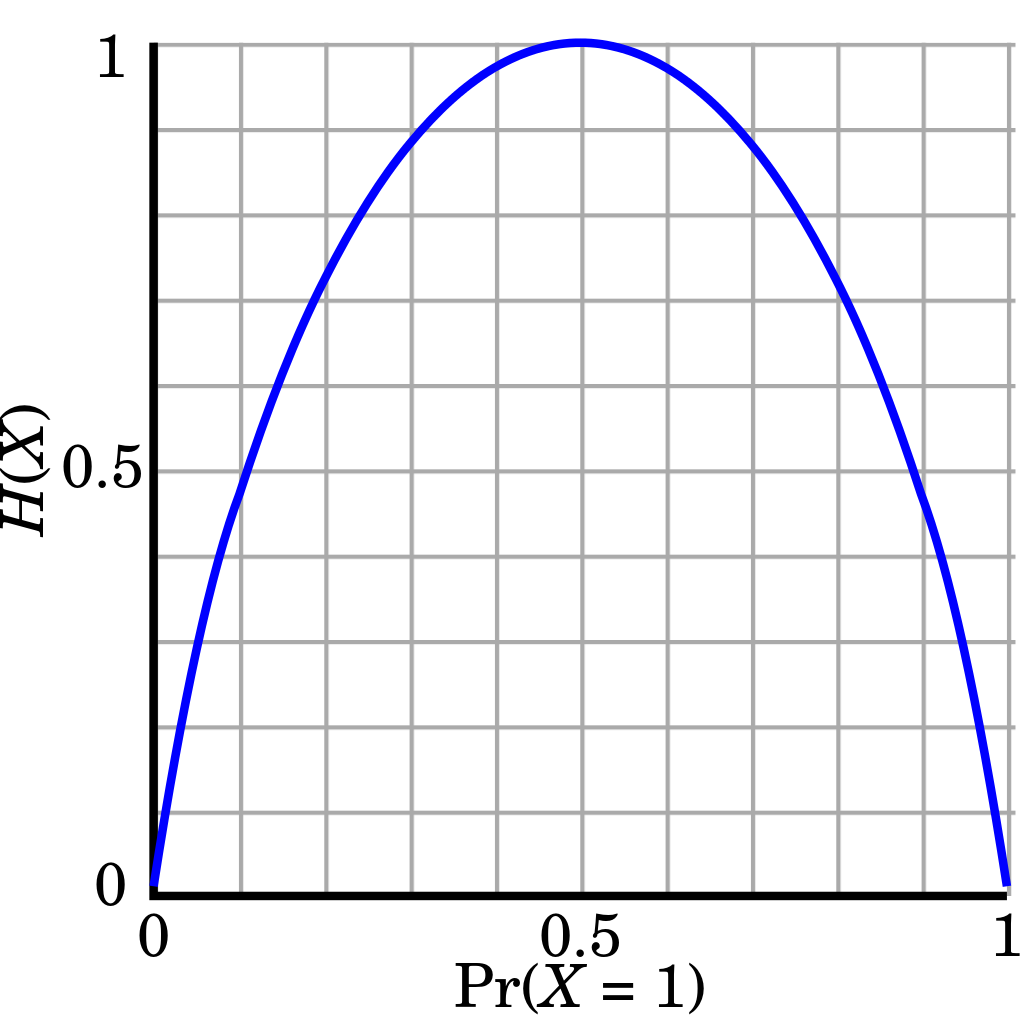
\includegraphics[width=0.5\textwidth]{figs/entropy.png}
    \caption{هنگامی $p=1$ است هیچ اطلاعات غیر قابل پیش‌بینی بدست نمی‌آید و مقدار انتروپی برابر با صفر است. به بیانی دیگر با احتمال یک می‌دانیم که $X=1$ خواهد بود و هیج عدم قطعیتی نداریم.
    از طرفی هنگامی که $p=0$ باشد باز هیچ اطلاعات ارزشمند و غیر منتظره‌ای بدست‌ نیامده چرا که این بار با احتمال یک می‌دانیم که $X=0$ است و در نتیجه انتروپی دوباره برابر با صفر خواهد شد.
    بیشترین عدم قطعیت یا انتروپی را هنگامی خواهیم داشت که $p=0.5$ باشد.
    در این حالت نمی‌توانیم هیچ تفاوتی میان رویدادهای مختلف قائل شویم و بیشترین عدم قطعیت و انتروپی هنگامی رخ می‌دهد که توزیع احتمالی یکنواخت باشد.}
    \label{fig:entropy}
\end{figure}

\subsection{انتروپی توام}

 انتروپی توام\LTRfootnote{joint entropy} دو متغیر تصادفی نظیر $X$ و $ِY$ برابر است با:
\begin{align*}
    H(X,Y) = \mathbb{E}\left[-\log p(x,y)\right] = - \sum_{x\in \mathcal{X},~ y \in \mathcal{Y}}p(x,y) \log p(x,y) 
\end{align*}
اگر $X$ و $Y$ از هم مستقل باشند می‌توان این رابطه را به صورت زیر نوشت:
\begin{align*}
    H(X,Y) =  - \sum_{x\in \mathcal{X},~ y \in \mathcal{Y}}p(x)p(y) \log \left[p(x)p(y) \right] = H(X) + H(Y)
\end{align*}

\subsection{انتروپی شرطی}

انتروپی شرطی\LTRfootnote{conditional entropy} یا عدم قطعیت متغیر تصادفی $X$ به شرط $Y$ برابر است با:
\begin{align*}
    H(X|Y) = \mathbb{E}_Y\left[H(X|y)\right] = -\sum_{y\in \mathcal{Y}}p(y)\sum_{x\in \mathcal{X}}p(x|y)\log p(x|y)= - \sum_{x\in \mathcal{X},~ y \in \mathcal{Y}}p(x,y) \log p(x|y) 
\end{align*}
که این رابطه را به صورت زیر نیز می‌توان نوشت:
\begin{align*}
    H(X|Y) =  - \sum_{x\in \mathcal{X},~ y \in \mathcal{Y}}p(x,y) \log \frac{p(x,y)}{p(y)} = H(X,Y) - H(Y)
\end{align*}

\subsection{کسب اطلاعات}

میزان کسب اطلاعات از یک متغیر تصادفی نظیر $X$ به شرط مشاهده (یادگیری) ویژگی $a$ برابر است با:
\begin{align*}
    IG(X,a):= H(X) - H(X|a)
\end{align*}
در واقع در اینجا می‌خواهیم بدانیم با دانستن و یا یادگیری یک ویژگی مانند $a$ میزان عدم قطعیت ما نسبت به $X$ به چه میزان کاهش می‌یابد. برای مثال اگر این دو از یکدیگر مستقل باشند در این صورت کسب اطلاعات برابر با صفر می‌شود.
این رابطه‌ را می‌توان به صورت واگرایی $\text{\begin{latin}
    KL
\end{latin}}$
نیز بیان کرد. فرض کنید دو توزیع احتمالاتی گسسته $P$ و $ْQ$ هر دو بر روی یک فضای نمونه نظیر $\mathcal{X}$ تعریف شده باشند، در این صورت داریم:
\begin{align*}
    D_\text{\begin{latin}KL\end{latin}}(P \| Q) = \sum_{x\in \mathcal{X}}P(x) \log \frac{P(x)}{Q(x)} = -\sum_{x\in \mathcal{X}} P(X)\log Q(x) - H(P)
\end{align*}
دقت داشته باشید که رابطه فوق نامتقارن بوده و در حالت کلی $D_\text{\begin{latin}KL\end{latin}}(P\|Q)\ne D_\text{\begin{latin}KL\end{latin}}(Q\|P)$ است. گاهی عبارت $-\sum_{x\in \mathcal{X}} P(X)\log Q(x)$ را به صورت $H(P,Q)$ نمایش می‌دهند که گرچه مانند انتروپی توام است، اما تعریف آن فرق می‌کند و به آن $\text{\begin{latin}
    cross-entropy
\end{latin}}$ می‌گویند. بنابراین این رابطه به صورت زیر نیز نمایش داده‌ می‌شود:
\begin{align*}
    D_\text{\begin{latin}KL\end{latin}}(P \| Q) = H(P,Q) - H(P)
\end{align*}
که باز هم تاکید می‌شود در این رابطه عبارت $H(P,Q)$ همان $\text{\begin{latin}
    cross-entropy
\end{latin}}$ بوده و به انتروپی توام ربطی ندارد.

\subsection{اطلاعات مشترک}

اطلاعات مشترک معیاری برای محاسبه میزان وابستگی دو متغیر و به بیانی دیگر نشان دهنده‌ی مقدار اطلاعات بدست آمده در رابطه با یک متغیر تصادفی به شرط مشاهده‌ی دیگری است که به صورت زیر تعریف می‌شود:
\begin{align*}
    I(X,Y) := \sum_{x\in \mathcal{X},~y\in \mathcal{Y}}p(x,y) \log \frac{p(x,y)}{p(x)p(y)} = H(X) - H(Y|X) 
\end{align*}
در نظر داشته باشید که این رابطه متقارن است:
\begin{align*}
    I(X,Y) = H(X) - H(X|Y) = H(Y) - H(Y|X) = I(Y,X)
\end{align*}